\documentclass[spanish, handout]{beamer}

\usepackage[utf8]{inputenc}
\usepackage[spanish, mexico]{babel}
\usepackage{hyperref}
\usepackage{xcolor}
\usepackage{color}
\usepackage{ragged2e}
\usepackage{tikz}
\usepackage{mathrsfs}
\usepackage{textcomp}

\usetikzlibrary{arrows, automata, positioning, fit, shapes.geometric, backgrounds}
\tikzset{%
    automaton/.style={->, >=stealth', shorten >=1pt, auto, semithick, initial text=$ $}
}

% \usepackage{courier}
% \usepackage{subfigure}
% \usepackage{enumerate}
% \usepackage{algorithmic}
% \usepackage{algorithm}


% \usepackage{listings}
% \usepackage{lstlinebgrd}

\newcommand\blfootnote[1]{%
\begingroup
\renewcommand\thefootnote{}\footnote{#1}%
\addtocounter{footnote}{-1}%
\endgroup
}

\usetheme{Boadilla}
%\usecolortheme{default}
\usefonttheme[onlymath]{serif}
\useoutertheme{infolines}

% Sets the templates

\definecolor{navyblue}{RGB}{0, 0, 128}

\setbeamertemplate{navigation symbols}{}
%\setbeamertemplate{headline}{}
\setbeamertemplate{footline}[frame number]
\setbeamertemplate{bibliography item}[text]
\setbeamertemplate{theorems}[numbered]

\setbeamercolor{title}{fg = navyblue, bg = white}
\setbeamercolor{frametitle}{fg = navyblue, bg = white}
\setbeamercolor{structure}{fg = navyblue}
\setbeamercolor{button}{fg = white,bg = navyblue}

\setbeamercovered{transparent}

\title{Autómatas de Pila (APs)}
\subtitle{Matemáticas Computacionales \\ (TC2020)}
\author{
\texorpdfstring{
\begin{center}
    M.C. Xavier Sánchez Díaz \\
    \href{mailto:sax@itesm.mx}{\texttt{sax@itesm.mx}}
\end{center}
}
{M.C. Xavier Sánchez Díaz}
}

\institute[Tecnológico de Monterrey]{
\includegraphics[scale=0.5]{../img/logo}}
\date{}

\begin{document}


\setlength{\rightskip}{0pt}

\begin{frame}[plain]
\titlepage
\end{frame}

% \begin{frame}{Tabla de contenidos}
% \tableofcontents
% \end{frame}

\section{Descripción informal de un AP}

\begin{frame}{¿Autómatas de Pila?}{Descripción informal de un AP}
    Un Autómata de Pila (AP) es un Autómata pero con una Pila (duh). \pause

    \bigskip

    El autómata tiene una \alert{pila}, la cual sirve como \textbf{memoria} extra para poder hacer operaciones más complicadas. \pause

    \bigskip

    Los \alert{Autómatas de Pila} son \textbf{equivalentes} a las \alert{Gramáticas Libres de Contexto}---sirven para representar lenguajes libres de contexto.
    
\end{frame}

\begin{frame}{¿Qué es un Autómata de Pila?}{Descripción informal de un AP}
    \begin{center}
        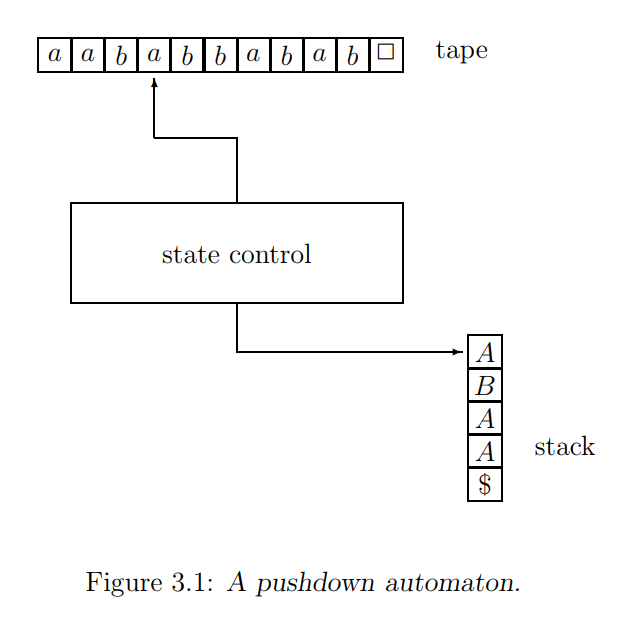
\includegraphics[width=0.57\textwidth]{../img/12-PDA.png} \blfootnote{Imagen de Maheshwari and Smid's \textit{Theory of Computation}, 2017}
    \end{center} 
\end{frame}

\begin{frame}{¿Qué es un Autómata de Pila?}{Descripción informal de un AP}
    Un AP tiene varios elementos:
    \bigskip

    \textbf{1)} Una \alert{cinta} dividida en \textbf{celdas} \pause
    
    \begin{itemize}
        \item Cada celda contiene un \textbf{símbolo} de la palabra de entrada el cual pertenece a un \textbf{alfabeto} $\Sigma$. \pause
        \item  Al final de la cinta, tenemos un \textbf{símbolo nuevo} para representar el \alert{final de la palabra}: $\square$. Este nuevo símbolo no pertenece al alfabeto de la palabra. \pause
    \end{itemize}

    \textbf{2)} Un \alert{cabezal en la cinta} que puede leer el valor de la celda en la que está, y que puede efectuar dos acciones $\sigma = \{N,R\}$: $N$ si no se mueve y $R$ si se mueve a la derecha. \pause

    \begin{center}
        \visible<5>{%
            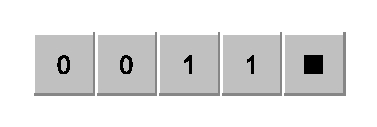
\includegraphics[width=0.5\textwidth]{../img/12-tape.pdf}
        }
    \end{center}
\end{frame}

\begin{frame}{¿Qué es un Autómata de Pila?}{Descripción informal de un AP}

    \textbf{3)} Una \alert{pila} que puede guardar símbolos. \pause

    \begin{itemize}
        \item Los símbolos que pueden almacenarse en la pila pertenecen a \textbf{otro alfabeto}: $\Gamma$. \pause
        \item Uno de estos símbolos es $\$$, el cual sí está \textbf{dentro del alfabeto de la pila}. \pause
    \end{itemize}

    \bigskip

    \textbf{4)} Un \alert{cabezal en la pila} el cual lee \textbf{el último símbolo} de la misma. \pause

    \begin{itemize}
        \item El cabezal puede \textit{apilar} (\alert{\texttt{push}}) más símbolos, o bien \textit{retirar} el símbolo de hasta arriba (\alert{\texttt{pop}}). \pause
    \end{itemize}

    \bigskip

    \textbf{5)} Un conjunto de \alert{estados}, unidos por \alert{transiciones} que dependen de los símbolos leídos por \textbf{ambos cabezales}.

\end{frame}

\begin{frame}{Una pila como estructura de datos}{Descripción informal de un AP}

    Una \alert{pila} (en inglés \textit{stack}) funciona por medio del principio \alert{LIFO}, que significa \textit{Last In, First Out}---el último elemento en entrar es el primero en salir. \pause

    \bigskip

    \begin{exampleblock}{Ejemplo}
        Sean $A$ una pila con los valores $A = \langle 1, 2, 3 \rangle$ y $F = \{\mathtt{pop}, \mathtt{push}\}$ un conjunto de funciones \textit{in-place} aplicables a pilas.
    \end{exampleblock} \pause

    \bigskip

    Si aplicamos la función \texttt{pop} sobre $A$, entonces obtendremos el valor $3$, y la pila pasará a ser $A = \langle 1,2 \rangle$. \pause

    \bigskip
    
    Si después metemos un valor más---digamos $4$---a la pila (proceso para el cual usamos la función \texttt{push}), entonces la pila es ahora $A = \langle 1, 2, 4 \rangle$. \pause

    \bigskip
    
    ¿Qué pasa si aplicamos \texttt{pop} nuevamente?
\end{frame}

\section{Formalización y diseño de APs}

\begin{frame}{Definiciones formales}{Formalización y diseño de APs}
    Hay \textbf{muchas} maneras de expresar los APs y sus elementos: \pause
    \begin{itemize}
        \itemsep1.5ex
        \item Brena (2003) utiliza transiciones expresadas en términos del input y \texttt{pop} y \texttt{push} de la pila, pertenecientes a una \textit{relación de transición}, con estados finales y nuevos símbolos. \pause
        \item Maheshwari y Smid (2017) utilizan una función de transición \textbf{completa} en términos del estado, el input, movimiento en la cinta ($\sigma = \{N,R\}$) y la función \texttt{replace} de la pila, sin estados finales. \pause
        \item Tinelli (2016) utiliza transiciones expresadas en términos del input y la función \texttt{replace} de la pila, con estados finales. 
    \end{itemize} \pause

    \bigskip

    Nosotros usaremos \textbf{una combinación de los tres}: diseñamos usando la notación de Maheshwari y Smid, refinamos usando la notación de Brena y con los símbolos de Tinelli \pause {\tiny because we're cool like that}.
\end{frame}

\begin{frame}{Definición Formal}{Formalización y diseño de APs}
    \begin{block}{Definición de un Autómata de Pila}
        Un autómata de pila $M$ es una tupla de la forma $M = (Q, \Sigma, \Gamma, \delta, q, F)$ donde: \pause
        \begin{itemize}
            \item $Q$ es un conjunto finito de \textbf{estados}, \pause
            \item $\Sigma$ es el \textbf{alfabeto de la cinta} (sin incluir $\square$), \pause
            \item $\Gamma$ es el \textbf{alfabeto de la pila} (incluyendo $\$$), \pause
            \item $q \in Q$ es el \textbf{estado inicial}, \pause
            \item $F \subseteq Q$ es un conjunto finito de \textbf{estados finales} y \pause
            \item $\delta$ es la función de transición.
        \end{itemize}
    \end{block}
\end{frame}

\begin{frame}{Definición Formal}{Formalización y diseño de APs}
    La función de transición $d$ es una función de la forma:
        \[\delta : \alert<3>{Q} \times (\alert<4>{\Sigma \cup \{\square\}}) \times \alert<5>{\Gamma} \to \alert<6>{Q} \times \alert<7>{\{N,R\}} \times \alert<8>{\Gamma^*}\] \pause
        \vspace{-1.5ex}
    \begin{exampleblock}{Ejemplo}
        Podemos escribir $\alert<3>{q_0} \alert<4>{1} \alert<5>{S} \to \alert<6>{q_1} \alert<7>{R} \alert<8>{SS}$ que significaría que: \pause
        \begin{itemize}
            \item Estando en el estado $\alert<3>{q_0}$, \pause
            \item al recibir un $\alert<4>{1}$, \pause
            \item y si el tope de la pila tiene $\alert<5>{S}$ \pause
        \end{itemize}
        entonces el AP
        \begin{itemize}
            \item cambia al estado $\alert<6>{q_1}$, \pause
            \item mueve la cinta hacia la derecha ($\alert<7>{R}$ight) y \pause
            \item reemplaza el tope de la pila por $\alert<8>{SS}$.
        \end{itemize}
    \end{exampleblock}
\end{frame}

{%
\setbeamersize{description width=-\labelsep}
\begin{frame}{Consideraciones adicionales}{Formalización y diseño de APs}
    \begin{description}
        \itemsep1.5ex
        \item[Configuración inicial] \hfill \\ 
        \begin{itemize}
            \item El AP empieza en el estado $q$. \pause 
            \item El cabezal de la cinta empieza en el símbolo inicial de la palabra $w$. \pause 
            \item La pila empieza con un solo símbolo, $\$$. \pause 
        \end{itemize}

        \item[Cómputo y terminación] \hfill \\ 
        El AP hace una serie de pasos de cómputo y \textit{termina} en el momento en que la pila se vacía. Si la pila no se vacía, entonces el programa no termina (\textit{loop} infinito). \pause 
        \item[Aceptación] \hfill \\ 
        El AP acepta la palabra $w$ si se cumplen las condiciones siguientes:
        \begin{enumerate}
            \item el autómata termina, y \pause 
            \item al momento de terminar, (i.e. la pila se vacía) el cabezal de la cinta está en el símbolo $\square$.
        \end{enumerate}
    \end{description}
\end{frame}
}

\begin{frame}{Ejemplo: \textit{Matching Parentheses}}{Formalización y diseño de APs}
    \textbf{Ejemplos de palabras aceptadas}: $(), ((())), ()(), \dots$ \pause

    \textbf{Estructura}:
    \begin{itemize}
        \item Antes de terminar de leer toda la palabra, la cantidad de ``('' debe ser mayor o igual que ``)'', y \pause
        \item Al terminar de leer toda la palabra, el número de ``('' debe ser igual al número de ``)''. \pause
    \end{itemize}

    Para no complicarnos, usaremos $a$ para representar ``('' y $b$ para representar ``)'' en la cinta. \pause

    \bigskip
    
    Por cada $a$ leída, metemos una $S$ en la pila. \pause
    Por cada $b$ que se lea, sacamos entonces una $S$.  \pause
    ¿Cuántos estados necesitamos? ¿Cuáles son finales? \pause

    Es un proceso \textbf{complicado}, por lo que se sugiere primero definir el AP formalmente (e.g. la función de transición completa, y parte por parte), y luego pasarlo a un diagrama con una relación de transición más pequeña: $Q \times \Sigma \cup \{\square\} \times \Gamma  \to Q \times \Gamma^*$.
    
    ¿Por qué no consideramos si se mueve o no se mueve el cabezal de la cinta?
\end{frame}

\begin{frame}{Ejemplo: \textit{Matching Parentheses}}{Formalización y diseño de APs}

    $M = (Q, \Sigma, \Gamma, \delta, q, F)$:

    \begin{columns}
        \begin{column}{0.4\textwidth}
            \begin{itemize}
                \item $Q = \{q_0, q_1\}$
                \item $\Sigma = \{a,b\}$
                \item $\Gamma = \{\$, S\}$
                \item $\delta =$
                \begin{itemize}
                    \item $((q_0,a,\$)(q_0,\$S))$
                    \item $((q_0,a,S)(q_0,SS))$
                    \item $((q_0,b,S)(q_0,\varepsilon))$
                    \item $((q_0,\square,\$),(q_1,\varepsilon))$
                \end{itemize}
                \item $q = q_0$
                \item $F = \{q_1\}$
            \end{itemize}
        \end{column}
        \begin{column}{0.6\textwidth}
            \begin{tikzpicture}[node distance=3cm, automaton]
                \node[state, initial] (q0) {$q_0$};
                \node[state, accepting] (q1) [right of=q0] {$q_1$};
    
                \path
                (q0) edge [loop above] node {$(a,\$,\$S), (a,S,SS), (b,S,\varepsilon)$} (q0)
                (q0) edge node {$\square,\$,\varepsilon$} (q1);
            \end{tikzpicture}
        \end{column}
    \end{columns}
    
\end{frame}

\begin{frame}{Ejemplo: $\{0^n1^n\}$}{Formalización y diseño de APs}

    $M = (Q, \Sigma, \Gamma, \delta, q, F)$:

    \begin{columns}
        \begin{column}{0.4\textwidth}
            \begin{itemize}
                \item $Q = \{q_0, q_1\}$
                \item $\Sigma = \{0, 1\}$
                \item $\Gamma = \{\$, S\}$
                \item $\delta =$
                \begin{itemize}
                    \item $((q_0,0,\$)(q_0,\$S))$
                    \item $((q_0,0,S)(q_0,SS))$
                    \item $((q_0,1,S)(q_1,\varepsilon))$
                    \item $((q_0,\square,\$),(q_1,\varepsilon))$
                    \item $((q_1,1,S)(q_1,\varepsilon))$
                    \item $((q_1,\square,\$)(q_1,\varepsilon))$
                \end{itemize}
                \item $q = q_0$
                \item $F = \{q_1\}$
            \end{itemize}
        \end{column}
        \begin{column}{0.6\textwidth}
            \begin{tikzpicture}[node distance=3.7cm, automaton]
                \node[state, initial] (q0) {$q_0$};
                \node[state, accepting] (q1) [right of=q0] {$q_1$};
    
                \path
                (q0) edge [loop above] node {$(0,\$,\$S), (0,S,SS)$} (q0)
                (q0) edge node {$(1,S,\varepsilon), (\square,\$,\varepsilon)$} (q1)
                (q1) edge [loop below] node {$(1,S,\varepsilon), (\square,\$,\varepsilon)$} (q1);
            \end{tikzpicture}
        \end{column}
    \end{columns}
\end{frame}

\begin{frame}{Combinación y concatenación}{Formalización y diseño de APs}
    \begin{description}
        \itemsep2.5ex
        \item[Combinación de APs] \hfill \\
        De manera muy similar a unir dos AFNs, la idea es hacer un estado inicial \textbf{previo} que una los estados iniciales de los APs usando transiciones vacías ($\varepsilon,\varepsilon,\varepsilon$). \pause
        \item[Concatenación de APs]  \hfill \\
        La concatenación funciona de manera muy similar que como era en AFNs, sin embargo hay que garantizar que la pila se encuentra en \textit{ciertas condiciones} antes de pasar al siguiente AP.
        La solución es utilizar un símbolo especial antes de iniciar con el primer AP, y sacarlo antes de iniciar la operación con el segundo.
    \end{description}
    
\end{frame}
% \section*{Referencias}
% \begin{frame}[t]{Referencias}
% \nocite{bibID01}
% \nocite{bibID02}

% \bibliographystyle{IEEE}
% \bibliography{biblio}
% \end{frame}

\end{document}